\documentclass[11pt,a4paper,openany,oneside,parskip=half*]{article}

\usepackage[utf8]{inputenc}
\usepackage{tocloft}
\usepackage{nomencl}
\usepackage{pdfpages}
\usepackage{scrextend}
\usepackage{bm}
\usepackage{cite}
\usepackage{amsmath}
\usepackage{graphicx}
\usepackage[justification=justified]{caption}
\usepackage{float}
\usepackage{multicol}
\usepackage{float}
\usepackage[section]{placeins}
\usepackage[english, ngerman]{babel} 
\usepackage{geometry} %Gr�ߟe des Bodys innerhalb der Seite 
\usepackage[utf8]{inputenc} 
\usepackage{ifthen}
\usepackage{caption}
\usepackage{multirow}
\usepackage{subfig}
%bindet die benutzten Packages ein

\linespread{1.25}

\captionsetup{width=0.485\linewidth}

\RequirePackage{ifthen}
\renewcommand{\nomgroup}[1]{%
  \ifthenelse{\equal{#1}{R}}{\item[\textbf{Roman Symbols}]}{%
    \ifthenelse{\equal{#1}{G}}{\item[\textbf{Greek Symbols}]}{%
      \ifthenelse{\equal{#1}{O}}{\item[\textbf{Operators}]}{%
	\ifthenelse{\equal{#1}{A}}{\item[\textbf{Acronyms}]}{%
	  \ifthenelse{\equal{#1}{S}}{\item[\textbf{Subscripts}]}{}}}}}}%
	
\renewcommand*\vec[1]{\boldsymbol{#1}}
\renewcommand*\matrix[1]{\boldsymbol{#1}}

\captionsetup[figure]{font=footnotesize}

\cftsetindents{section}{0em}{2.65em}   
\cftsetindents{subsection}{1.5em}{3em}   
\cftsetindents{subsubsection}{2.5em}{3.5em}
%setzt die fettgedruckte Schreibweise fuer Vektoren und Matrizen

\geometry{top=3cm, bottom=4cm}
\geometry{bindingoffset=1.5cm} %offset zum binden
\newcommand{\HRule}{\rule{\linewidth}{0.5mm}}  % definere gerade Linie mit 0.5mm Dicke

\makeindex %

\begin{document}
\begin{titlepage}
\begin{figure}[htp]
\vspace*{-3cm} 
\hspace*{2.7cm}  

\includegraphics{./Titelseite/rwth_aia_en_rgb.eps}
\end{figure}
\begin{center}
\textbf{Diese Arbeit wurde vorgelegt am Aerodynamischen Institut}
\end{center}
\begin{center} % ab hier zentriert
\vspace*{4.2cm} %lasse 4.5 cm Platz von oben
{ \huge \bfseries Investigations on two-way coupling effects of particle-laden decaying isotropic turbulent flows}\\[0.3cm] % Groߟe Buchstaben, fett gedruckt, lasse 0.3cm Platz nach unten
\HRule \\[0.5cm] %Linie, 0,5cm Platz nach unten
\textsc{\Large{Projektarbeit}}\\ %in Kapitälchen
\textsc{\Large{von}}\\
\textsc{\LARGE{Julian Stemmermann, Steffen Trienekens und Christian Soika}}\\[0.5cm]
\HRule \\[0.4cm]
{\Large{Aerodynamisches Institut der RWTH Aachen}}\\[.5cm]
\begin{otherlanguage}{ngerman}
{\large \today} \\[1.5cm] % heutiges Datum
\end{otherlanguage}
\vfill % So viel Platz lassen, dass es bis zur Ende der Seite geht, wobei die Abstände bei dem nächsten vfill gleich sind
\begin{flushleft} \large  %Einrückung, groß
\begin{tabular}{ll} % Tabelle
Betreuer: &Konstantin Fr\"ohlich \\
Erstpr\"ufer: &Univ.-Prof.\,Dr.-Ing. Wolfgang Schr\"oder
\end{tabular}
\end{flushleft}
\vfill % So viel Platz lassen, dass es bis zur Ende der Seite geht
\end{center}
\end{titlepage}

\numberwithin{equation}{section} %bestimmt die Nummerierung der Gleichungen, in diesem Fall nach Kapitel anstatt sie einfach durchzunummerieren

\makenomenclature %erstellt und druckt die Nomenklatur-Tabelle


\renewcommand{\refname}{}
\renewcommand{\nomname}{}



\setlength{\columnsep}{30pt}
\setlength{\parindent}{0pt}

\pagebreak
\tableofcontents{} %erstellt die Inhaltsangabe
\thispagestyle{empty}
\pagebreak

\renewcommand{\thesection}{\Roman{section}}
\pagenumbering{Roman} 

%Nomenclature
\nomenclature[sinftyref]{$\infty, \mathrm{ref}$}{Referential variables}
\nomenclature[sp]{p}{Particle-concerning variables}
\nomenclature[sl]{$\lambda$}{Taylor-microscale variables}
\nomenclature[sL]{L}{Variables regarding the integral lengthscale}
\nomenclature[sz]{$0$}{Starting values of the variable}
\nomenclature[sn]{n}{Variable at n-th timestep}
\nomenclature[snn]{$\mathrm{n+1}$}{Variable at (n+1)-th timestep}
\nomenclature[sf]{f}{Fluid-concerning variables}
\nomenclature[rK(t)]{$K(t)$}{History kernel}
\nomenclature[geps]{$\epsilon$}{Viscous dissipation rate}
\nomenclature[rUx]{$\bar U(\vec{x})$}{Filtered velocity field}
\nomenclature[gW]{$\phi(\mathrm{Re_p})$}{Empirical drag correction factor}
\nomenclature[arms]{rms}{Root mean square}
\nomenclature[aCPP]{CPP}{Computational point particles}
\nomenclature[aDNS]{DNS}{Direct numerical simulation}
\nomenclature[aLES]{LES}{Large-eddy simulation}
\nomenclature[asgs]{sgs}{Subgrid scale}
\nomenclature[asP]{sP}{Single-phase simulation}
\nomenclature[aPP]{PP}{Particle-laden simulation}
\nomenclature[aILES]{ILES}{Implicit large-eddy simulation}
\nomenclature[oN]{$\vec\nabla$}{Nabla operator} 
\nomenclature[rQ]{$\vec{Q}$}{Vector of conservative Eulerian variables}
\nomenclature[rH]{$\vec{\bar{H}}$}{Flux tensor}
\nomenclature[gr]{$\rho$}{Fluid density}
\nomenclature[ru]{$\vec{u}$}{Fluid velocity}
\nomenclature[rE]{$E$}{Specific inner energy}
\nomenclature[rHi]{$\vec{\bar{H}^\mathrm{i}}$}{Inviscid part of the flux tensor}
\nomenclature[rHv]{$\vec{\bar{H}^\mathrm{v}}$}{Viscous part of the flux tensor}
\nomenclature[rp]{$p$}{Pressure}
\nomenclature[rRe]{$Re$}{Reynolds number}
\nomenclature[gt]{$\matrix{\bar{\tau}}$}{Stress tensor}
\nomenclature[rq]{$\vec{q}$}{Heat conduction vector}
\nomenclature[gg]{$\gamma$}{Isentropic exponent}
\nomenclature[re]{$e$}{Specific internal energy}
\nomenclature[rPr]{$Pr$}{Prandtl number}
\nomenclature[gm]{$\mu$}{Dynamic viscosity}
\nomenclature[rcp]{$c_\mathrm{p}$}{Specific isobaric heat capacity}
\nomenclature[rcv]{$c_\mathrm{v}$}{Specific isochoric heat capacity}
\nomenclature[rkt]{$k_\mathrm{t}$}{Thermal conductivity}
\nomenclature[rI]{$\matrix{\bar{I}}$}{Identity tensor}
\nomenclature[rS]{$\vec{\bar{S}}$}{Rate-of-strain tensor}
\nomenclature[rT]{$T$}{Temperature}
\nomenclature[rS]{$S$}{Sutherland temperature}
\nomenclature[rR]{$R$}{Specific gas constant}
\nomenclature[rx]{$\vec{x}$}{Position vector}
\nomenclature[rt]{$t$}{time}
\nomenclature[gtL]{$\tau_\mathrm{L}$}{Eddy turnover time}
\nomenclature[rL]{$L$}{Integral length scale}
\nomenclature[rU]{$U$}{Characteristic fluid velocity}
\nomenclature[gh]{$\eta$}{Kolmogorov length scale}
\nomenclature[gh0]{$\eta_\mathrm{0}$}{Initial Kolmogorov length scale}
\nomenclature[gth]{$\tau_{\mathrm{\eta}}$}{Kolmogorov time scale}
\nomenclature[rF]{$\vec{F}$}{Force vector per unit volume of the particle acting on the fluid}
\nomenclature[rFn]{$\vec{F}_\mathrm{pp}$}{Sum vector of forces acting on the particles}
\nomenclature[rVp]{$\mathrm{V}_\mathrm{p}$}{Particle volume}
\nomenclature[rVf]{$\mathrm{V}_\mathrm{f}$}{Fluid volume}
\nomenclature[rRep]{$Re_\mathrm{p}$}{Particle Reynolds number}
\nomenclature[gnu]{$\nu$}{Kinematic viscosity}
\nomenclature[rdp]{$d_\mathrm{p}$}{Particle diameter}
\nomenclature[grp]{$\rho_\mathrm{p}$}{Particle density}
\nomenclature[rxp]{$\vec{x}_\mathrm{p}$}{Particle position vector}
\nomenclature[rvp]{$\vec{v}_\mathrm{p}$}{Particle velocity vector}
\nomenclature[gmc]{$\lambda_\mathrm{c}$}{Ratio of physical point particles to computational point particles}
\nomenclature[rnp]{$N_\mathrm{p}$}{Number of physical point particles}
\nomenclature[rnc]{$N_\mathrm{c}$}{Number of computational point particles}
\nomenclature[gpsi]{$\Psi$}{Integral coupling rate}
\nomenclature[geps]{$\vec{\varepsilon}$}{Integral dissipation rate}
\nomenclature[gpsip]{$\Psi_\mathrm{p}$}{Coupling rate for one particle}
\nomenclature[gpsipp]{$\Psi_\mathrm{pp}$}{Integral coupling rate using the point-particle approach}
\nomenclature[gtp]{$\tau_\mathrm{p}$}{Particle response time}
\nomenclature[gD]{$\Delta$}{Cell length}
\nomenclature[rdi]{$d_\mathrm{i}$}{Distance between particle position and cell center}
\nomenclature[gphiv]{$\phi_\mathrm{v}$}{Volume fraction}
\nomenclature[gphim]{$\phi_\mathrm{m}$}{Mass fraction}
\nomenclature[gYf]{$\Upsilon_\mathrm{f}$}{Fluid domain without particle surroundings}
\nomenclature[gepss]{$\vec{\bar{\varepsilon}}$}{Integral dissipation rate of the flow field}
\nomenclature[geps']{$\vec{\varepsilon}'$}{Additional integral particle induced dissipation rate}
\nomenclature[odelta1]{$\delta$}{Small step of the following variable}
\nomenclature[od]{$\frac{\mathrm{d}}{\mathrm{d}t}$}{Material derivative}
\nomenclature[oD]{$\frac{\mathrm{D}}{\mathrm{D}t}$}{Time derivative following a fluid unit}
\nomenclature[odelta2]{$\frac{\partial{}}{\partial{t}}$}{Partial derivative with respect to time}
\nomenclature[oO]{$\vec{:}$}{Inner tensor product}
\nomenclature[rn]{$\vec{n}$}{Normal vector}
\nomenclature[rA]{$A$}{Control surface}
\nomenclature[rap]{$\vec{a}_\mathrm{p}$}{Particle acceleration}
\nomenclature[gsigma]{$\sigma$}{Smoothing parameter}
\nomenclature[rEk]{$E_\mathrm{k}$}{Turbulent kinetic energy of the fluid}
\nomenclature[rFp]{$\vec{F}_\mathrm{p}$}{Particle surface force vector}
\nomenclature[rTp]{$\vec{T}_\mathrm{p}$}{Particle torque vector}
\nomenclature[gwp]{$\vec{\omega}_\mathrm{p}$}{Particle angular velocity vector}
\nomenclature[rEkB]{$E_\mathrm{kB}$}{Turbulent kinetic energy of the particles}
\nomenclature[rt*]{$t^\mathrm{*}$}{Time normalized by initial eddy turnover time}
\nomenclature[rup]{$\vec{u}_\mathrm{p}$}{Vector of fluid velocity at the particle position}
\nomenclature[rV]{$V$}{Control volume}
\nomenclature[rN]{$N$}{Grid refinement of the simulation}
\nomenclature[rG(r)]{$G(r)$}{Homogeneous filter function}
\nomenclature[ru']{$\vec{u}'$}{Vector of fluid velocity fluctuations}
\nomenclature[rmp]{$m_\mathrm{p}$}{Particle mass}
\nomenclature[rmf]{$m_\mathrm{f}$}{Fluid mass}
\nomenclature[rR(r,t)]{$R (r, t)$}{Two-point correlation}
%Nomenclature

\setlength{\nomitemsep}{-\parsep}

\section{Nomenclature}
\vspace*{-1.2cm}
\printnomenclature[1.5cm]
\pagebreak
\renewcommand{\thesection}{\arabic{section}}
\setcounter{section}{0}
\section{Introduction}
\pagenumbering{arabic}
\setcounter{page}{1}
\begin{figure}[h]
	\centering
  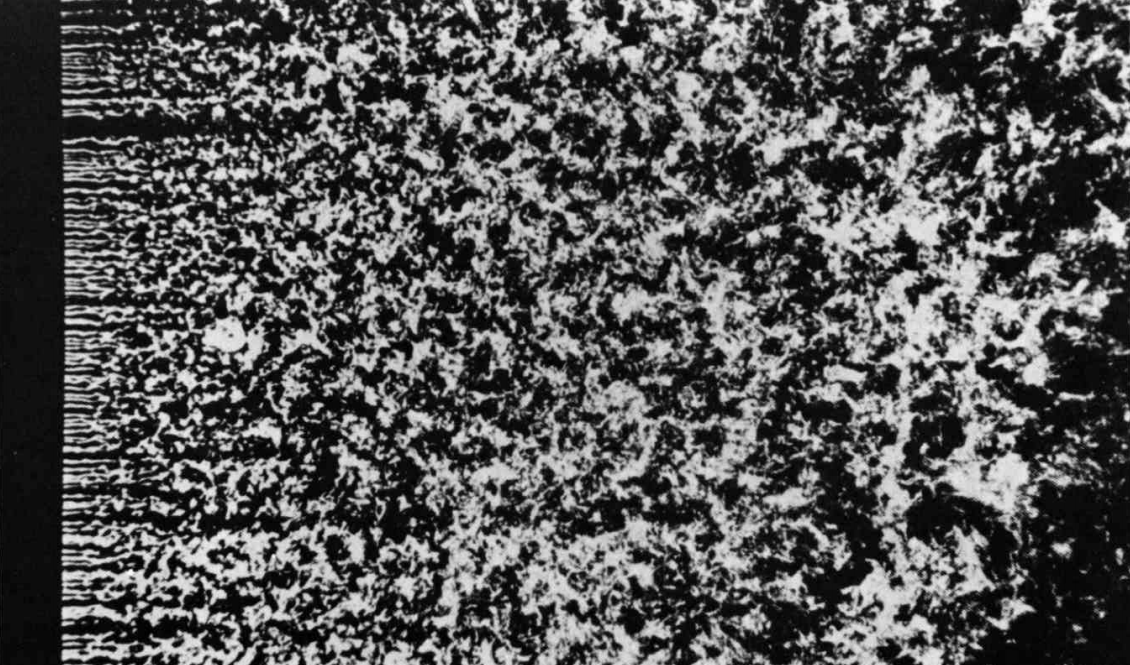
\includegraphics[width=\textwidth]{./Abbildungen/TurbulentMotion_Introduction.png}
  \captionsetup{width=0.97\linewidth}
	\caption{Photograph courtesy of Hassan Nagib and Thomas Corke. Formation of a nearly isotropic turbulent flow field behind a grid \cite{albumOfFluidMotion}.}
	\label{introduction_picture}
\end{figure}
Particle-laden turbulent flows are ubiquitous in nature.
Spray automization in fuel injectors, cyclonic particle separation in oil refineries and sediment accumulation in pipelines are examples for technical applications, where it is of huge interest to predict the impact of the particles on turbulent flows.
Turbulence augmentation or attenuation by particles is therefore a decisive factor.
\newline
A study about the impact of particles on the isotropic decaying turbulent flow is presented.
Incompressible, isothermal and isotropic decaying turbulence will serve as the carrier flow. Gravity is omitted to avoid prominent directions. Isotropic turbulence is a relatively good assumption when a small region of a high-Reynolds-number flow, which is not affected by boundary effects, is observed \cite{Kolmogorov1941}. This fact is visualized by Fig \ref{introduction_picture}. Describing turbulent flows is a difficultsgs task because of the involvement of many different scales of turbulent motion.
\newline
In this work the influence of the particles on the isotropic decaying turbulence is numerically calculated by using direct numerical (DNS) and large-eddy simulations (LES). Direct numerical simulations are able to resolve all scales of turbulent motion due to their high grid refinement. Large-eddy simulations have a lower grid resolution and use therefore a subgrid-scale model (sgs) to model these scales. This type of simulation therefore has a lower computational effort.
\newline
The simulations were carried out using the point-particle approach, where each particle is tracked via a Langrangian approach. The feedback of the particles on the flow field is modeled by sources and sinks, which is referred to as two-way coupling. Alternatives are one-way coupling, at which only the flow exerts influence on the particles, and four-way coupling, which extends two-way coupling by particle-particle interactions. Two-way coupling is fitting for the simulations in this study, because the volume fraction $\phi_\mathrm{v}= 10^{-3}$ of the particles is large enough to alter the turbulence. Volume fractions below $\phi_\mathrm{v}= 10^{-6}$ are referred to as one-way coupling and the interactions that can be observed at values greater than $\phi_\mathrm{v}= 10^{-3}$ are attributed to four-way coupling \cite{particleladenTurbulentFlows:DirectSimulationAndClosureModels}\cite{OnPredictingParticle-LadenTurbulentFlows}.
The particle diameter is defined to be smaller than the Kolmogorov scale, i.e. the smallest scale of the turbulent flow. The particle density is much higher than the fluid density.
\newline
To lower the computational effort in general, a new variable, which describes the fraction of physical to numerical point particles, is introduced and validated.
\newline
In the following the structure of this work is described. 
First, mathematical models for single-phase and particle dynamics are given. 
Additionally, the scales of turbulent motion are described.
Subsequently, the used discretization method to integrate the particle tracking equations is described and the 'computational point particles', in the following referred to as CPP, are introduced.
Thereafter, the computational basics of both DNS and LES and their respective advantages and disadvantages are explained. 
The CPP approach is validated by analyzing turbulent kinetic energy budgets for LES and DNS. For this purpose a test is conducted at first to find out which number of CPPs is appropriate for further evaluation.
Also the number of particles that is needed to get consistent averaged values for the flow characteristics is investigated.
Finally, a short conclusion is given.
\pagebreak
\section{Mathematical models}
In this section the Navier-Stokes equations in integral formulation, the characteristic turbulent scales and the kinematic and dynamic equations for the particle phase are introduced.
\newline
\subsection{Equations governing the fluid phase}
The conservation of mass, momentum and energy for a control volume V reads
\begin{equation} \label{NavierStokes}
  \int\limits_V \frac{\partial{\vec{Q}}}{\partial{t}} \, \mathrm{d} V+ \int\limits_{\partial{V}} \vec{\bar{H}} \cdot \vec{n} \, \mathrm{d} A = \vec0
\end{equation}
with time $t$ and the flux tensor $ \vec{\bar{H}} $.
The vector $ \vec{Q} $ contains the variables fluid density $ \rho $, 
fluid velocity $ \vec{u} $ and specific inner energy $ E $: 
\begin{equation}
 \vec{Q}= \left( \begin{array}{c}\rho\\\rho \vec{u}\\\rho E \end{array} \right).
\end{equation}
$\vec{\bar{H}} $ is the flux tensor which contains the inviscid and viscous flux, i.e.
\begin{equation} 
\vec{\bar{H}} = \vec{\bar{H}^\mathrm{i}} + \vec{\bar{H}^\mathrm{v}} = 
 \left( \begin{array}{c}\rho \vec{u}\\\rho \vec{u} \vec{u} + p\\\vec{u} (\rho E + p) \end{array} \right) - 
 \frac{1}{Re} \left( \begin{array}{c}\ 0 \\ \matrix{\bar{\tau}}\\ \matrix{\bar{\tau}} \vec{u} + \vec{q} \end{array} \right),
\end{equation} 
with the shear stress $\matrix{\bar{\tau}}$, heat conduction $\vec{q}$ and the pressure p. The Reynolds number 
$ Re = \frac{\rho_\infty u_\infty l_\mathrm{ref}}{\mu_\infty} $ is defined to be the ratio of inertia forces to viscous forces with reference density $\rho_\infty$, velocity $u_\infty$, length $l_\mathrm{ref}$ and dynamic viscosity $\mu_\infty$. 
\newline
The specific inner energy $ E $ 
and the heat conduction $ \vec{q}$ are defined as
\begin{equation}
 E = e  \frac{1}{2} \vec{|u|}^2 \, \mathrm{and}
\end{equation}
\begin{equation}
 \vec{q} = - \frac{\mu}{Pr (\gamma - 1)} \vec\nabla T,
\end{equation}
with the constant capacity ratio $\gamma = \frac{c_p}{c_v}$ and the Prandtl number
$ Pr = \frac{\mu_\infty c_\mathrm{p}}{k_\mathrm{t}}$
using the specific heat capacities of the fluid $ c_\mathrm{v} $ and $ c_\mathrm{p} $ and thermal conductivity $k_\mathrm{t}$.
Assuming that the fluid is newtonian, the Stokes hypothesis yields
\begin{equation}
 \matrix{\bar{\tau}} = 2 \mu \matrix{\bar{S}} - \frac{2}{3} \mu (\vec\nabla \cdot \vec{u}) \matrix{\bar{I}},
\end{equation}
in which $ \matrix{\bar{S}} = \frac{(\vec\nabla \vec{u})(\vec\nabla \vec{u})^T}{2} $ denotes the rate-of-strain tensor. Additionally, the viscosity
$ \mu $ can be approximated by Sutherland's law
\begin{equation}
 \mu (T) = \mu_\infty \biggl(\frac{T}{T_\infty}\biggl)^{3/2} \frac{T_\infty + S}{T + S},
\end{equation}
where S is the Sutherland temperature.
To achieve closure the caloric state equation $ e = c_\mathrm{v} T $ and the state equation for an ideal gas $
p = \rho R T $ are used. The specific gas constant is determined by $ R = c_\mathrm{p} - c_\mathrm{v} $. 
\newline
\subsection{Scales of turbulent flows}
Turbulent flows can be described as a superposition of chaotic, three-dimensional vortical structures of various scales, referred to as eddies. Larger eddies decay and pass their kinetic energy down to smaller scales. At the smallest scales, the kinetic energy finally dissipates into heat due to the viscous dissipation. This behavior is called the 'energy cascade' and was first described by Richardson \cite{Richardson1920} and quantified by Kolmogorov \cite{Kolmogorov1941}.
\newline
Considering homogeneous isotropic turbulence, with zero mean velocity and the integral dissipation rate $\varepsilon$, the characteristic length scales of a turbulent flow can be defined by the two-point correlation $R$, which is the normalized product of the velocity's fluctuation $u'$ at two different positions 
$\vec{x}$ and $\vec{x} + \vec{e}r$ at the same time $t$
\begin{equation}
R (r, t) = \frac{\overline{u'(\vec{x}, t)u'(\vec{x} + \vec{e}r, t)}}{\overline{u'^2}},
\end{equation}
as
\begin{equation}
 \frac{1}{\lambda^2} = -\frac{1}{2}\biggl(\frac{\partial^2 R}{\partial r^2}\Bigr|_{\substack{r=0}}\biggl),
\end{equation}
\begin{equation}
\lambda = \sqrt{15 \frac{\nu}{\varepsilon}} u'
\end{equation}
or
\begin{equation} \label{eq:integralLengthScale}
L = \int_{0}^{\infty} R (r, t)  \, \mathrm{d}r
\end{equation}
with $\lambda$ being the Taylor microscale, $L$ the integral length scale, $u'$ denoting the absolute value of the velocity's fluctuation and $\vec{e}$ pointing in the same direction as $\vec{u'}$ with $|\vec{e}| = 1$.
\newline
The Taylor microscale can be used to compute the Taylor-scale Reynolds number
\begin{equation}
Re_\mathrm{\lambda} = \frac{u' \lambda}{\nu}.
\end{equation}
\newline
$L$ and the corresponding timescale $\tau_\mathrm{L}$, which is mostly called 'eddy turnover time', describe the large eddies. At these scales the energy is brought into the flow, creating the 'energy-containing range'. The eddy turnover time is defined by
\begin{equation}
\tau_\mathrm{L} = \frac{L}{U},
\end{equation}
with the characteristic fluid velocity $U$.
\newline
The smallest scales in a turbulent flow are the Kolmogorov length $\eta$ and time scale $\tau_\mathrm{\eta}$. At these scales, the effects of viscosity take place and the energy dissipates into heat. With the estimate $\varepsilon \approx \frac{U^3}{L} $ they can be written as
\begin{equation}
\eta = \biggl (\frac{\nu^3 L}{U^3} \biggl )^{1/4}
\end{equation}
and
\begin{equation}
\tau_\mathrm{\eta} = \biggl (\frac{\nu L}{U^3} \biggl ).
\end{equation}
Both these scales are coupled by the Reynolds numbers
\begin{equation}
\frac{L}{\eta} = Re^{3/4}
\end{equation}
and
\begin{equation}
\frac{\tau_\mathrm{L}}{\tau_\mathrm{\eta}} = {Re_\mathrm{L}}^{1/2}
\end{equation}
with $Re_\mathrm{L} = \frac{u' L}{\nu}$.
It can be observed from these equations that the spacing between the scales increases for higher Reynolds numbers. 
\newline
\subsection{Particle dynamics} %Steffen

$\vec{F}_\mathrm{pp}$ is the sum of several pressure and shear forces acting on the particles and is described explicitly by the Maxey-Riley equation \cite{EquationOfMotionForASmallRigidSphereInANonuniformFlow}.
Reduced to the governing forces and with neglection of gravity the dynamic equation of the particles becomes
\begin{multline} \label{navier_stokes_particle}
 \vec{F}_\mathrm{pp} = m_\mathrm{p} \frac{\mathrm{d}\vec{v}_\mathrm{p}}{\mathrm{d}t} =\rho V_\mathrm{p}\frac{\mathrm{D}\vec{u}_\mathrm{p}}{\mathrm{D}t} + 3 \pi \mu d_\mathrm{p}(\vec{u}_\mathrm{p}-\vec{v}_\mathrm{p})\phi(Re_\mathrm{p})+ \frac{1}{2}\rho \mathrm{V}_\mathrm{p} \biggl(\frac{\mathrm{D}\vec{u}_\mathrm{p}}{\mathrm{D}t}-\frac{\mathrm{d}\vec{v}_\mathrm{p}}{\mathrm{d}t}\biggl) +
\\ 3 \pi \mu d_\mathrm{p}\int_{0}^{t} K(t) (t-t') \cdot \biggl(\frac{\mathrm{d}\vec{u}_\mathrm{p}}{\mathrm{d}t'}- \frac{\mathrm{d}\vec{v}_\mathrm{p}}{\mathrm{d}t'}\biggl)dt'.
\end{multline}
$\vec{v}_\mathrm{p}(\vec{x}_\mathrm{p},t)$ is the particle velocity vector with the time derivative $\mathrm{d}/\mathrm{d}t$ along the particle trajectory while $\mathrm{D}/\mathrm{D}t$  is the material derivative at one point. $\vec{u}_\mathrm{p}(t) = \vec{u}_\mathrm{p}(\vec{x}_\mathrm{p},t)$ is the velocity of the undisturbed fluid at the particle position $\vec{x}_\mathrm{p}$.
The individual forces on the right side of the equation are stated in the following:
\begin{itemize} 
\item  $\rho V_\mathrm{p}\frac{\mathrm{D}\vec{u}_\mathrm{p}}{\mathrm{D}t}$: \newline
pressure gradient of the undisturbed flow
\item $3 \pi \mu d_\mathrm{p}(\vec{u}_\mathrm{p}-\vec{v}_\mathrm{p})\phi(Re_\mathrm{p}):$\newline
quasi-steady Stokes drag that is parallel to the undisturbed streamlines and is described by the Stokes' law as the force of viscosity acting on the interface of small spherical particles and fluid that can be achieved at very low Reynolds numbers in a viscous fluid

\item $\frac{1}{2}\rho \mathrm{V}_\mathrm{p} \biggl(\frac{\mathrm{D}\vec{u}_\mathrm{p}}{\mathrm{D}t}-\frac{\mathrm{d}\vec{v}_\mathrm{p}}{\mathrm{d}t}\biggl)$:
\newline
added mass force, representing the influence of the fluid's inertia that has an impact on the particle, in case of a different acceleration than the particles
\item $3 \pi \mu d_\mathrm{p}\int_{0}^{t} K(t) (t-t') \cdot \biggl(\frac{\mathrm{d}\vec{u}_\mathrm{p}}{\mathrm{d}t'}- \frac{\mathrm{d}\vec{v}_\mathrm{p}}{\mathrm{d}t'}\biggl)dt'$: \newline
Basset history force taking the unsteady motion into account using a history kernel $K(t)$ 
\end{itemize}

\eqref{navier_stokes_particle} is based on Stokes flow conditions, i.e., vanishing particle Reynolds number $Re_\mathrm{p} \ll 1$. In addition in this thesis, particles with $d_\mathrm{p} \ll \eta$ are investigated.
As a result for heavy particles, the drag force is the dominating contributor of Eq. \eqref{navier_stokes_particle} as reported by \cite{TheImportanceOfTheFocusActingOnParticlesInTurbulentFlows}. Therefore $\vec{F}_\mathrm{pp}$ can be reduced to
\begin{equation} \label{kurze_Partikelgleichung}
\vec{F}_\mathrm{pp} =  m_\mathrm{p} \frac{\mathrm{d}\vec{v}_\mathrm{p}}{\mathrm{d}t} = 3 \pi \mu d_\mathrm{p}(\vec{u}_\mathrm{p}-\vec{v}_\mathrm{p})\phi(Re_\mathrm{p}).
\end{equation}
The empirical correction factor $\phi(Re_\mathrm{p}) = 1+0.15Re_\mathrm{p}^\mathrm{0.687}$ is used for finite $\mathrm{Re_\mathrm{p}}$. \newline Eq. \eqref{kurze_Partikelgleichung} can be reformulated to
\begin{equation} \label{shortPaticleDynamics}
\frac{\mathrm{d}\vec{v}_\mathrm{p}}{\mathrm{d}t} = \frac{\phi(Re_\mathrm{p})}{\tau_\mathrm{p}}(\vec{u}_\mathrm{p}-\vec{v}_\mathrm{p}),
\end{equation}
with the particle relaxation time $\tau_\mathrm{p}=\frac{1}{18}\frac{\rho_\mathrm{p}}{\rho}\frac{d_\mathrm{p}^\mathrm{2}}{\nu}$. 
\newline
Together with the kinematic equation    
\begin{equation}
 \frac{\mathrm{d}\vec{x}_\mathrm{p}}{\mathrm{d}t} = \vec{v}_\mathrm{p},
\end{equation}
the Eqs.  \eqref{NavierStokes} and \eqref{kurze_Partikelgleichung} form a closed system of equations.
\pagebreak
\section{Numerical methods} %Julian
Two numerical methods are discussed and their main differences pointed out in the following chapter, the DNS (direct numerical simulation) and the LES (large-eddy simulation). The basis of both are the Navier-Stokes equations as described above. The simulations were carried out using ZFS, the simulation tool developed and implemented at the Institute of Aerodynamics at RWTH Aachen University 
\cite{anAdaptiveMultilevelMultigridFormulationForCartesianHierarchicalGridMethods} \cite{aStrictlyConservativeCartesianCutCellMethodForCompressibleViscousFlowsOnAdaptiveGrids}. 
The tool is capable of simulating compressible finite-volume flows using unstructured Cartesian grids.
\newline
\subsection{Discretization of the particle dynamics}
To compute the Lagrangian particle trajectories, a predictor-corrector scheme based on the trapezoidal rule for numerical integration
\begin{equation}
f (t + \delta t) \approx f(t) + \frac{\delta t}{2} \left[ \frac{\partial f(t)}{\partial t} + \frac{\partial f(t + \delta t)}{\partial t} \right ]
\end{equation}
is used.
\newline
The first step is the prediction of the new particle position $\vec{x}_{\mathrm{p}, n+1}$ using a Taylor expansion for a small time step $\delta t$
\begin{equation}
\vec{x}_{\mathrm{p}, n+1} = \vec{x}_{\mathrm{p}, n} + \delta t \vec{v}_{\mathrm{p}, n} + \frac{1}{2} \delta t^2 \vec{a}_{\mathrm{p}, n},
\end{equation}
with $\vec{a}_{\mathrm{p}, n}$ particle acceleration, where the subscript $\mathrm{p}$ denotes the particle and the subscript $n$ the time step.
\newline
To avoid filtering effects, the fluid velocity $\vec{u}_{\mathrm{p}, n+1}$ at the particle position $\vec{x}_{\mathrm{p}, n+1}$ is set equal to the nearest cell fluid velocity. 
\newline
The predicted velocity and acceleration are calculated with
\begin{equation}
\vec{v}_{\mathrm{p}, n+1} = \frac{\vec{v}_\mathrm{p,n} + \frac{1}{2} \delta t \left(\vec{a}_{\mathrm{p, n}} + \frac{f_\mathrm{d}}{\tau_\mathrm{p}}\vec{u}_{\mathrm{p}, n+1} \right)}{1 + \frac{1}{2} \frac{f_\mathrm{D}}{\tau_\mathrm{p}} \delta t},
\end{equation}
\begin{equation}
\vec{a}_{\mathrm{p}, n+1} = \frac{\frac{f_\mathrm{D}}{\tau_\mathrm{p}} \left(\vec{u}_{\mathrm{p}, n+1} - \vec{v}_{\mathrm{p}, n} - \frac{1}{2} \delta t \vec{a}_{\mathrm{p}, n} \right)}{1 + \frac{1}{2} \frac{f_\mathrm{D}}{\tau_\mathrm{p}} \delta t}.
\end{equation}
The updated particle position must be corrected by an additional term according to the trapezoidal rule
\begin{equation}
\vec{x}_{\mathrm{p}, n+1} = \vec{x}_{\mathrm{p}, n} + \frac{1}{2} \delta t \left( \vec{v}_{\mathrm{p}, n+1} + \vec{v}_{\mathrm{p}, n} \right) + \frac{1}{12} \delta t^2 \left( \vec{a}_{\mathrm{p}, n+1} - \vec{a}_{\mathrm{p}, n} \right).
\end{equation}
\newline
These approaches to compute the particle trajectories require a lot of computational resources. 
\newline
Due to reduce this requirement the creation of numerical clusters of point particles is considered. For this purpose the ratio $\lambda_\mathrm{c}$ of physical point particles $N_\mathrm{p}$ to CPPs $N_\mathrm{c}$ is introduced ($\lambda_\mathrm{c} = \frac{N_\mathrm{p}}{N_\mathrm{c}}$). To compensate this lack of particles, the feedback force is multiplied by $\lambda_\mathrm{c}$, due to the $\lambda_\mathrm{c}$-fold mass of the (cluster-)particles.
\newline
To model the impact of the particles on the fluid, the Navier-Stokes equations \eqref{NavierStokes} are extended by momentum sources or sinks. The feedback force of the particles is exerted on the fluid using a distance based weighting function
\begin{equation}
\vec{F} = \vec{F}_\mathrm{pp} \cdot \frac{\mathrm{e}^{- \big(d_\mathrm{i}^\mathrm{2}/(\sigma \Delta^\mathrm{2})\big)}}{\sum \limits_{i} e^{- \big(d_\mathrm{i}^\mathrm{2}/(\sigma \Delta^\mathrm{2}) \big)}},
\end{equation}
with the distance between particle postion and the cell center $d_\mathrm{i}$, the grid width $\Delta$, and a smoothing parameter $\sigma$ that controls the distribution of $\vec{F}$ on the adjacent cells.
\newline
\subsection{Direct numerical simulation}
With DNS, the Navier-Stokes equations are solved completely. This provides a very accurate result, as all scales of motion are being resolved. Hence it requires an immense level of computational resources which increases rapidly with the Reynolds number: $N \propto Re_{\mathrm{\lambda}}^{9/2}$ with the gridsize N of the simulation. With the LES, as described below, the computational effort is 99.98 \% less compared to DNS, which is the fraction of the dissipative scale. This leaves 0.02 \% of the flow, which is correlative with the fraction of the energy-containing larger-scale \cite{turbulentFlows}.
\newline
\subsection{Large-eddy simulation}
\begin{figure}[h]
    \centering
    \begin{minipage}[t]{.5\textwidth}
        \centering
        \subfloat[]{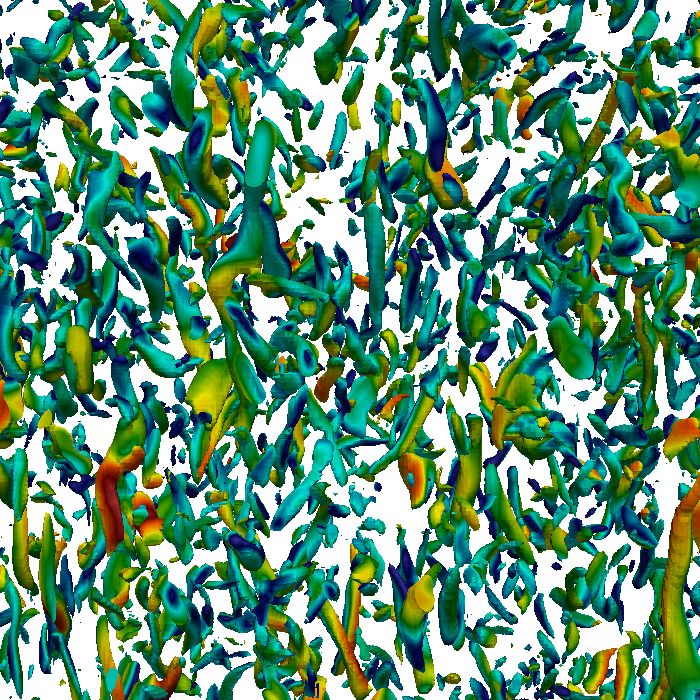
\includegraphics[width=0.95\linewidth]{./Abbildungen/256_velocity_4.png}}
        \label{256_velocity}
    \end{minipage}%
    \begin{minipage}[t]{0.5\textwidth}
        \centering
        \subfloat[]{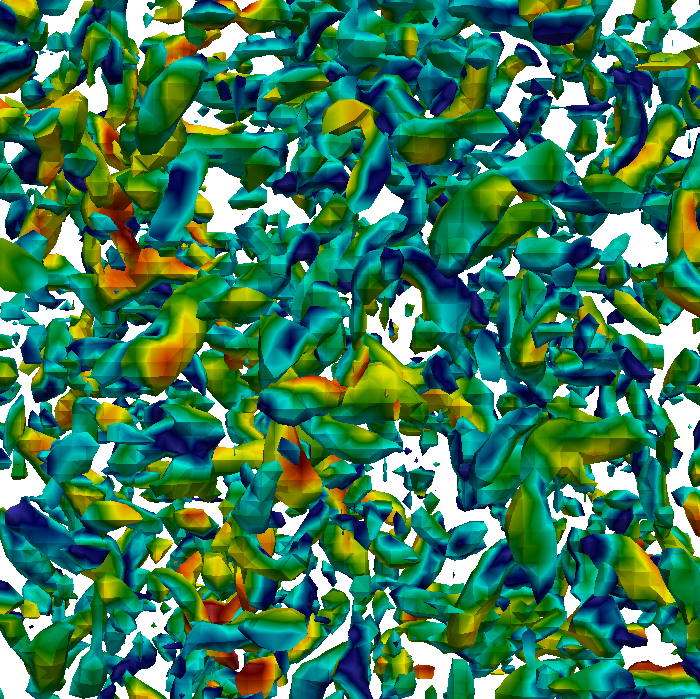
\includegraphics[width=0.95\linewidth]{./Abbildungen/64_velocity.png}}
        \label{64_velocity}
    \end{minipage}
    \captionsetup{width=0.97\linewidth}
\caption{Instantaneous snapshot of the parallel projection of an isotropic decaying turbulent flow field computed by a DNS (a) and a $\mathrm{LES_{64}}$ (b). 'Worm-like' structures in an isotropic turbulent flow field. The more refined grid on the left shows more and better resolved structures, while the right picture reveals more artificially generated artifacts. For details on creation, see Appendix A.}
\label{comparisonLESDNS}
\end{figure}
Due to the fact that DNS is effortful, LES was created to save time and resources. The energy containing large scales are completely resolved and the impact of the small scales on the large scales are modeled.
\newline
Simulating only the larger-scale motions is called filtering, which means that the smaller-scale motions, also known as fluctuation, are filtered out. The filtered velocity field is calculated by 
\begin{equation}
\bar U(\vec{x}) = \int_{-\infty}^{\infty} G(\vec{r})U(\vec{x} - \vec{r})  \, \mathrm{d}\vec{r},
\end{equation}
with $G(\vec{r}) $ being a homogeneous filter function \cite{turbulentFlows}. To model the filtered smaller-scale motions a subgrid-scale (sgs) model is necessary. According to Hickel (2007) the interference between explicit sgs and the truncation error can be exploited, i.e. the truncation error can serve as model of the effects of unresolved scales, which is therefore an implicit sgs model. Thus it is called implicit LES (ILES) \cite{implicitLES}.
\newline
Even though the small scales are modeled in the LES, the effects of filtering can be seen in figure \ref{comparisonLESDNS}.
\newline
\pagebreak
\section{Results}
In this section, the properties and results of the DNS and LES of particle-laden decaying isotropic turbulence which have been carried out will be presented. An additional test to find out which  number of CPPs could be used is presented. Special emphasis will be put on the turbulent kinetic energy budgets and their use to interpret the findings.
\newline
\subsection{Turbulence modulation by particles}
The particle-laden turbulence modulation by particles in decaying isotropic turbulence is determined by the coupling rate $\Psi$, which describes the energy transfer between both fluid and particle phase, the background dissipation rate of the flow field $\bar{\varepsilon}$ and the particle-induced dissipation rate $\varepsilon'$. These variables together form an equation which describes the change in turbulent kinetic energy
\begin{equation}
\frac{\mathrm{d} E_\mathrm{k}}{\mathrm{d} t} = \Psi (t) - \bar{\varepsilon} (t) - \varepsilon' (t).
\end{equation}
As the dissipation rate is always of positive value, it acts as a sink for the fluid's turbulent kinetic energy. In difference to that, the coupling rate can serve either as source or sink, depending on the acceleration of the particles \cite{mechanismsoftwowaycoupling}. The coupling rate for fully resolved particles $\Psi$ is defined as
\begin{equation}
\Psi (t) = \sum_{p=1}^{N_\mathrm{p}} \Psi_\mathrm{p}= - \sum_{p=1}^{N_\mathrm{p}} (\vec{F}_\mathrm{p} \cdot \vec{v}_\mathrm{p} + \vec{T}_\mathrm{p} \cdot \vec{\omega}_\mathrm{p}),
\end{equation}
using surface force $\vec{F}_\mathrm{p}$, particle velocity $\vec{v}_\mathrm{p}$, torque $\vec{T}_\mathrm{p}$ and angular velocity $\vec{\omega}_\mathrm{p}$ to describe the transfer of kinetic energy resulting at each particle. 
\newline
As mentioned before, the flow field is considered nearly incompressible, therefore the equation  for the viscous dissipation rate can be approximated by
\begin{equation}
 \epsilon (t) \approx 2 \mu \vec{\bar{S}}\vec{:}\vec{\bar{S}},
\end{equation}
where $\vec{:}$ denotes the inner tensor product. This rate can then be integrated over the fluid domain excluding particles and their direct surroundings $\Upsilon_\mathrm{f}$, leading to the background flow field dissipation rate
\begin{equation}
\bar{\varepsilon} (t) = \int\limits_{\Upsilon_\mathrm{f}} \epsilon(t) \mathrm{d}V.
\end{equation}
Additionally the particles change the fluid's rate of dissipation due to their volume forces. The additional dissipation rate for fully resolved particles can be computed by
\begin{equation}
	\varepsilon' = \sum_{p=1}^{N_\mathrm{p}} \vec{F}_\mathrm{p} \cdot (\vec{u}_\mathrm{p}-\vec{v}_\mathrm{p})+ \vec{T}_\mathrm{p} \cdot (\vec{\Omega}_\mathrm{p} - \vec{\omega}_\mathrm{p}), \; \rho_\mathrm{p} \gg \rho,
\end{equation}
using the velocity of the fluid $\vec{u}_\mathrm{p}$ and the vorticity vector of the undisturbed flow around one particle $\vec{\Omega}_\mathrm{p}$, both at the particle position. Fluid inertia as well as hydrostatic and shear stresses were neglected in this study.
\newline
For $\rho_\mathrm{p} \gg \rho$ and the point-particle approach the coupling rate $\Psi$ and the additional dissipation rate $\varepsilon'$ are implicitly coupled. Torque and angular velocity were neglected for the used point-particle approach, leading to
\begin{equation}
\Psi_\mathrm{pp} (t) = \Psi - \varepsilon'(t) = - \sum_{p=1}^{N_\mathrm{p}} \vec{F}_\mathrm{p} \cdot \vec{u}_\mathrm{p}.
\end{equation}
This leads to 
\begin{equation}
\frac{\mathrm{d} E_\mathrm{k}}{\mathrm{d} t} = \Psi_\mathrm{pp} (t) - \bar{\varepsilon} (t) = - \sum_{p=1}^{N_\mathrm{p}} \vec{F}_\mathrm{p} \cdot \vec{u}_\mathrm{p} - \bar{\varepsilon} (t).
\end{equation}
\newline
\subsection{Simulation setup}
All cases were simulated on a cubic domain and a Cartesian grid using different grid refinement levels. For the LES-cases $64^3$, $96^3$ and $128^3$ are employed, hence the need to model smaller scales with sgs models, which have already been validated in \cite{ValidationOfParticleLadenLargeEddySimulationUsingHPCSystems}. For a DNS, $256^3$ cells are necessary to resolve all scales.
\newline
The particle-free case was initialized using a seed-based number random generator, a process which is described in detail in \cite{orszag1969numerical}. At the initial eddy turnover time $t^*=t\frac{\varepsilon_\mathrm{0}}{{u_\mathrm{0}}^2} \approx 0.27=t_\mathrm{inj}^*$, using the initial viscous dissipation rate $\varepsilon_\mathrm{0}$ and initial rms-velocity $u_\mathrm{0}$, a restart file is written out to initialize the subsequent simulation of the particle-laden isotropic turbulence.
\newline
This file is then used to set up a second simulation, where the particles are initialized with the fluid velocity at random positions. The single-phase DNS and particle-laden DNS will be used as reference for analyzing other results. The single-phase results will be in the following referred to as sP, and particle-laden results as PP. The PP simulations are set up to match the volume fraction $\phi_\mathrm{v}=\frac{V_\mathrm{p}}{V_\mathrm{f}}= 10^{-3}$ and mass fraction of $\phi_\mathrm{m}=\frac{m_\mathrm{p}}{m_\mathrm{f}}=1$. Hence the density ratio was $\frac{\rho_\mathrm{p}}{\rho} = 1000$ and the particle diameter is $d_\mathrm{p} \approx 0.6 \eta_\mathrm{0}$ with $\eta_\mathrm{0}$ being the initial Kolmogorov length. At the timestep of injection the Reynolds number of the Taylor microscale was $Re_\lambda \approx 58$. 
\newline
\subsection{Simulation results}
\begin{figure}[h]
    \centering
    \begin{minipage}{0.5\textwidth}
        \centering
 	   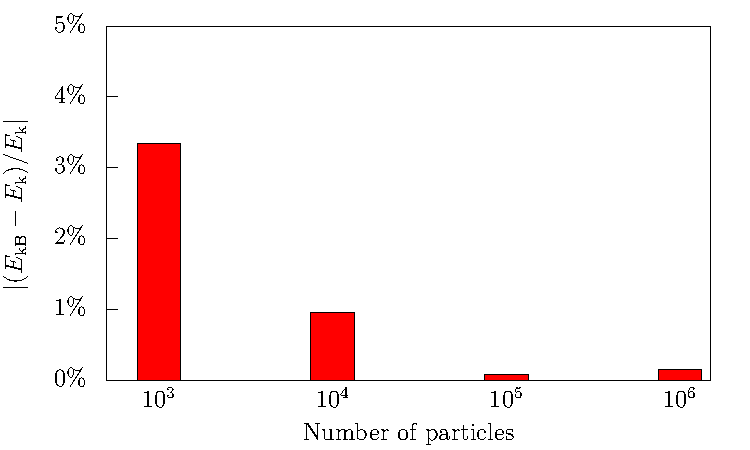
\includegraphics[width=\linewidth]{./Abbildungen/kineticEnergy_numberOfParticles.pdf}
    \end{minipage}%
        \begin{minipage}{0.5\textwidth}
        \centering
        \caption{Initializing different numbers of point-particles for a $\mathrm{LES_{128}}$. An inaccuracy can be observed for small numbers of particles. This behavior can be noticed for all other resolutions. The relative deviation of turbulent kinetic energy of particles and carrier flow is below 1\% for $10^4$ particles.}
	\label{kineticEnergy_numberofparticles}
    \end{minipage}
    \end{figure}
\begin{figure}[]
    \centering
    \begin{minipage}[t]{0.5\textwidth}
        \centering
 	   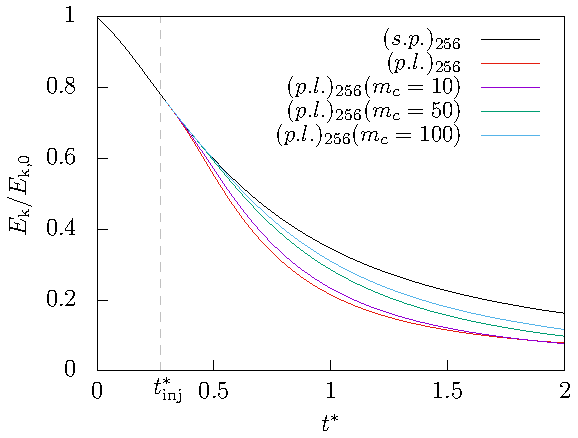
\includegraphics[width=\linewidth]{./Abbildungen/256/kineticEnergy_time.pdf}
	   \caption{Kinetic energy $E_\mathrm{k}$ normalized by its initial value $E_\mathrm{k,0}$ over time normalized by initial eddy turnover time. Shortly after the injection the PP-cases separates from the sP-flow. The higher-clustered cases show significant differences compared to the reference case PP-DNS.}
	\label{kineticEnergy_time_256}
    \end{minipage}%
\begin{minipage}[t]{0.5\textwidth}
        \centering
        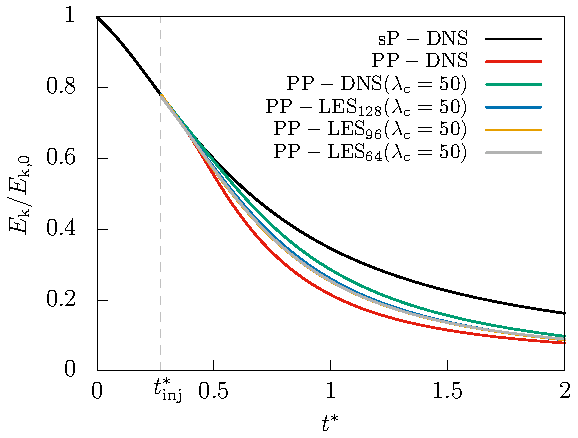
\includegraphics[width=\linewidth]{./Abbildungen/256/kineticEnergy_comp50.pdf}
        \caption{Kinetic energy $E_\mathrm{k}$ normalized by its initial value $E_\mathrm{k,0}$ over time normalized by initial eddy turnover time for different grid resolutions and with constant $\lambda_\mathrm{c}=50$. The lower-resolution simulation results are more similar to the particle-laden reference case PP-DNS.}
        \label{comparison_LES_DNS}
    \end{minipage}
\end{figure}
\begin{figure}[]
    \centering
    \begin{minipage}[t]{0.5\textwidth}
         \centering
        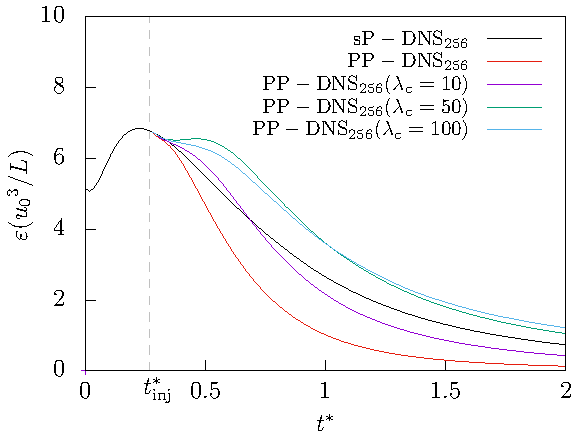
\includegraphics[width=\linewidth]{./Abbildungen/256/diss_time.pdf}
        \caption{Normalized dissipation rate $\bar{\vec{\varepsilon}}$ over time normalized by initial eddy turnover time. The unclustered PP-case shows a lower dissipation rate than the sP-case. Highly clustered PP-cases show a higher dissipation rate.}
        \label{diss_time_256}
    \end{minipage}%
    \begin{minipage}[t]{0.5\textwidth}
        \centering
        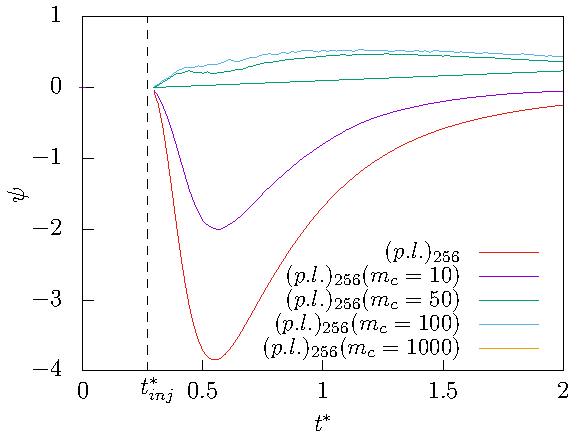
\includegraphics[width=\linewidth]{./Abbildungen/256/coupling_time.pdf}
        \caption{Normalized point-particle coupling rate $\Psi_\mathrm{pp}$ over time normalized by initial eddy turnover time. The PP-case without clustering shows the lowest coupling rate. Both highly-clustered PP-cases show physically questionable behavior.}
        \label{coupling_time_256}
    \end{minipage}
\end{figure}
The first set of simulation was set up to investigate how different numbers of injected particles have an influence on the difference of turbulent kinetic energy of both particle and fluid. As mathematical description of turbulent flows is based on statistics, small numbers of particles can lead to questionable results. 
\newline
An example for the deviation in kinetic energy for different numbers of particles can be found in Fig. \ref{kineticEnergy_numberofparticles}. The normalized difference in kinetic energy $E_\mathrm{kB}$ of the particles and the flow itself $E_\mathrm{k}$ shows a correlation between particle number and accuracy in this single simulation. One-time simulations in other grid sizes show similar results. 
\newline
This simulations served as test and a first evaluation, which number of CPPs are purposeful to simulate. As the flow statistics are relatively accurate for simulations with only $10^4$ particles, the method of CPPs could be a useful tool to lower computational effort. This leads to the assumption that simulations with a $\lambda_\mathrm{c}$ of 100 seem fitting with an overall number of a million particles. 
\newline
The second set of simulations of this study is set up to investigate the influence of CPPs on the accuracy of the simulations to find out which amount can be implemented without high loss in accuracy. For this purpose, the variable $\lambda_\mathrm{c}$, which was established before, was implemented in the program code. All simulations were then set up with the overall same number of a million particles, altering the CPPs. Simulations were conducted for $\lambda_\mathrm{c}=$10, 50 and 100. Additionally simulations of the single-phase flow and an unclustered particle-laden flow were conducted. A DNS serves as reference for later evaluations. 
\newline
It can be seen in Fig. \ref{kineticEnergy_time_256} that the decay in turbulent kinetic energy $E_\mathrm{k}$ normalized by initial turbulent kinetic Energy $E_\mathrm{k,0}$ from the injection point depends highly on the number of clustered particles. It can be stated that the flow's statistics for high $\lambda_\mathrm{c}$ converge towards the sP-case. 
\newline
As it can be seen in Fig. \ref{comparison_LES_DNS} the behavior of lower-resolution particle-laden simulations seems to be less prone to CPPs, as the lower-resolution simulations are more similar to the PP-DNS reference.
\newline
Figs. \ref{diss_time_256} and \ref{coupling_time_256} can be interpreted using the turbulent kinetic energy budget introduced earlier. The PP-case without clustering shows a lower dissipation rate (normalized with the referencial dissipation rate $\varepsilon_\mathrm{ref}=\frac{u_0^3}{L}$) than the sP-case. Both highly-clustered cases show a higher rate over the monitored period of time, which is an unphysical behavior. 
\newline
The coupling rate is negative the whole time for the PP-cases with lower $\lambda_\mathrm{c}$ and positive for the higher-clustered cases. The variables of the DNS and $\mathrm{LES_{64}}$ at $t^* \approx 1$ can be found in Tab.\ref{table_values_DNS_LES}. 
Being very similar in the time shortly after the injection, the flow statistics diverge for different $\lambda_\mathrm{c}$ in case of the DNS rapidly. For a high number of CPPs, the simulations drift away from the reference, leading even to unphysical behavior for $\lambda_\mathrm{c} \gg 50$. 
\begin{table}[]
	\begin{center}
	\begin{tabular}{| c | c l | c c c c c c c |}
	\hline
	Case & $\lambda_\mathrm{c}$& $\frac{m_\mathrm{c}}{m_\mathrm{V,cell}}$ &$\varepsilon \frac{L}{{u_0}^3}$ & $\frac{\lambda}{L}$ & $\frac{\eta}{L} $ & $Re_\lambda$ & $E_\mathrm{k}/E_\mathrm{k,0}$ & $E_\mathrm{kB}/E_\mathrm{k,0}$ & \\
	\hline
	\hline
	\multirow{4}{*}{DNS}
	&1 &16.78 & 0.97& 0.039 & 0.0032 & 38.73 & 0.21 & 0.29 &\\
	&10 &167.78 & 2.08 & 0.028 & 0.0026 & 28.66 & 0.23 & 0.34 &\\
	&50 &838.86 & 3.51 & 0.024 & 0.0023 & 27.31 & 0.28 & 0.52 &\\
	&100 &1677.72 & 3.51 & 0.025 & 0.0023 & 29.42 & 0.31 & 0.62 &\\
	\hline
	\hline
	\multirow{4}{*}{$\mathrm{LES_{64}}$}
	&1 & 0.26 & 0.74 & 0.046 & 0.0034 & 48.26 & 0.23 & 0.28 &\\
	&10 & 2.62 & 0.74 & 0.046 & 0.0034 & 48.13 & 0.23 & 0.28 &\\
	&50 & 13.11 & 0.90 & 0.044 & 0.0032 & 47.54 & 0.25 & 0.30 &\\
	&100 & 26.21 & 1.03 & 0.042 & 0.0031 & 47.60 & 0.27 & 0.30 &\\
	\hline
	\end{tabular}
	\captionsetup{width=0.9\linewidth}
	\caption{Variables of the simulations one turnover time after injection for two particle-laden simulations, PP-DNS and $\mathrm{PP-LES_{64}}$.}
	\label{table_values_DNS_LES}
	\end{center}
	\end{table}
In difference to that, the $\mathrm{LES_{64}}$ shows less impact to change in CPPs. 
\newline
In Fig. \ref{particlekineticenergy_time_256} the kinetic energy of the particles is displayed. For increasing $\lambda_\mathrm{c}$, the kinetic energy of the particles becomes smaller. This behavior leads to the assumption that the clustering produces the behavior of heavy particles as the results fit to the findings of Schneiders \cite{Schneiders2017}. 
\newline
Fig. \ref{vergleich_coupling_time_256} can be used to point out the difference in susceptibility for this method. It is evident that a correlation between inaccuracy of the simulations and the refinement level of the grid exists. For the same ratio of physical point particles to CPPs the results show different behavior depending on the grid refinement level. The unclustered PP-case is included as reference. It is therefore less critical to cluster particles in lower-resolution grids, although the results are not nearly as accurate as for the unclustered simulations. 
\begin{figure}[]
    \centering
     \begin{minipage}[t]{0.5\textwidth}
        \centering
        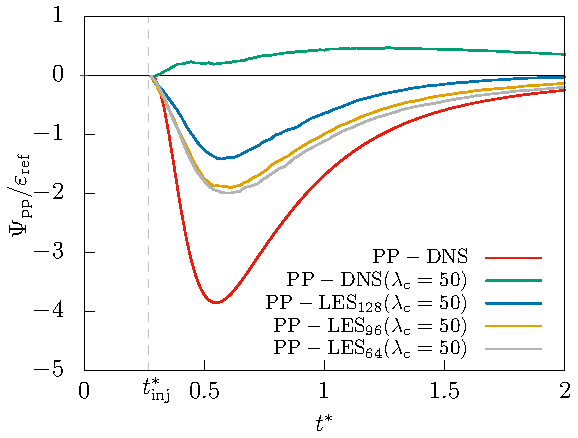
\includegraphics[width=\linewidth]{./Abbildungen/vergleich_coupling_time50.pdf}
        \caption{Point-particle coupling rate $\Psi_\mathrm{pp}$ with constant $\lambda_\mathrm{c}$ for various resolutions. A relation of resolution and accuracy can be observed.}
        \label{vergleich_coupling_time_256}
        \end{minipage}%
    \begin{minipage}[t]{.5\textwidth}
         \centering
        \includegraphics[width=\linewidth]{./Abbildungen/256/particlekineticenergy_time.pdf}
        \caption{Kinetic energy of the particles $E_\mathrm{kB}$ normalized by initial turbulent kinetic energy. The PP-case without clustering shows the biggest decay in kinetic energy. }
        \label{particlekineticenergy_time_256}
    \end{minipage}
\end{figure}
A correlation between the fraction of masses of one particle cluster to one cell can be observed in Tab. \ref{table_values_DNS_LES}. It seems to be the case that for increasing mass ratio of one cluster to one cell the simulation results become less accurate. This phenomenon was first described by Maxey and Patel \cite{maxey1997simulations}, as particle-induced point forces induce a vorticity to the flow at the particle position. Additionally they pointed out that a nonuniform particle distribution, caused by particle inertia or added mass, would have a larger impact on the turbulent kinetic energy of the carrier flow.
\newline 
The simulation on a $64^3$-grid is therefore less susceptible to altering the CPPs because the cells, and therefore the mass of one cell, are substantially bigger than in the $256^3$-grid for a constant domain size.
\pagebreak
\section{Conclusion and outlook}
In this study multiple simulations were carried out to evaluate a method for lowering computational effort. The statistics of simulations on various resolutions were compared and evaluated. CPPs have been validated to be a useful tool to achieve less computing time, if properly used.
\newline
The DNS showed to be prone for errors created by CPPs. Coupling and dissipation rate were affected very much by them, leading even to unphysical results. In contrast to that the coarser-grid simulations were less prone to CPPs, as multiple comparisons showed. The mass-fraction of one particle-cluster to the fluid content of one cell showed to be an important factor in statistical accuracy. This is because of self-induced disturbances of the particles. These particle clusters seem to behave like heavier particles, as comparisons with results from other literature show.
\newline
To enhance understanding and for future improvements of this method, further investigations are needed. There could be simulations to test which mass-fraction delivers sufficient precision while achieving the goal of less computational effort. For this task it is important to define the goal of future simulations of particle-laden isotropic decaying turbulence. For industrial application, a higher number of CPPs could be used, while in scientific work more accurate results are needed. 
\newline
%\subsection*{Acknowledgements}
%This work was supervised by Konstantin Fr\"ohlich, we would like to express our gratitude. Thank you for the chance of learning about turbulent flows and simulations, the advice and the deep insights in scientific work. We also appreciate the chance of writing this work at the Institute of Aerodynamics of the RWTH Aachen University.
\pagebreak
\section{References}
\vspace*{-1.2cm}
\nocite{*} %erm�glicht, dass auch Literatur, welche nicht zitiert wurde in der Bibliography auftaucht
\bibliography{Projektarbeit} %ruft die Bibliography-Datei auf
\bibliographystyle{plain} %setzt den Zitierstil
\pagebreak
\section{Appendix A}
\subsection*{Creating of pictures showing tubular structures}
The pictures used in to point out the differences between DNS and LES were generated using ParaView, an open-source-software developed by a joint-venture of Kitware and the Los Alamos National Laboratory. More information about the software can be found at www.paraview.org. To show the tubular structures in a turbulent flow, two filters were used: One was the AIALambda2Criterion1-Filter and the other one was the ISOVolume1-Filter. These filters were then set to visualize the velocity of the flow colored by magnitude. To diversify the different velocity-magnitudes, a rainbow-colorscheme was used. 
\end{document}
